\chapter{Wykorzystane biblioteki i narzędzia}

\section{ECLiPSe}

% SW: Powiedziałbym, że ECLiPSe to środowisko do wykonwania programów CLP (trudno powiedzieć, że służy do tworzenia aplikacji.
ECLiPSe\cite{EclipseSite} jest systemem typu open-source do wykonywania aplikacji wykorzystujących paradygmat programowania logicznego z ograniczeniami. System ten użyty został do testowania przykładowych procedur medycznych. 
% SW: Tutaj warto wyjaśnić, dlaczego nie zostało wykorzystane w systemie realizowanym w ramach pracy (np. z uwagi na ograniczaną możliwość intergracji z programami w języku Java).
Nie współpracuje natomiast z wykonanym w ramach pracy magisterskiej systemem, jest to odrębny program. 
% SW: Rozumiem, że tutaj pisze Pan o częściach głównego okna systemu ECLiPse -- sądzę, że należy to jasno powiedieć, a także zamieścić przykładowy ekran.
Okno systemu ECLiPSe składa się z trzech części. Pierwsza część służy do wprowadzania komend. Zamiast wprowadzania komend można wczytać gotowy program z pliku za pomocą polecenia Compile znajdującym się w menu File. Druga część programu wyświetla wyniki, trzecia natomiast pokazuje ewentualne błędy oraz inne komunikaty. Poniżej przedstawiono wygląd okna programu ECLiPSe.
\begin{figure}[H]
\centering
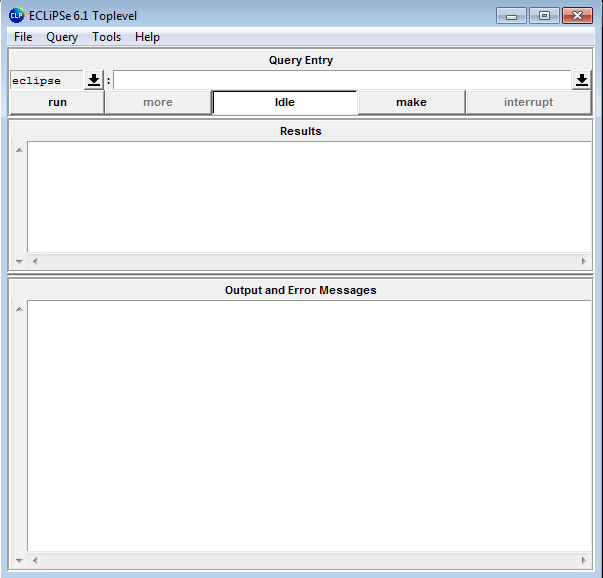
\includegraphics[width=0.7\textwidth]{img/okno.png}
\end{figure}


% SW: Taki fragmentaryczny opis składni jest mało przdatny. Napisałbym raczej, że przykładowy program przedstawiono w poprzedniej sekcji. Poza tym w poprzedniej sekcji umieściłbym tłumaczenia dotyczące interpretacji symboli "\#=" i "\#", ponieważ pojawiają się one w przykładowym programie.

%Komendy dla tego systemu składają się ze zdań zakończonych kropką, poszczególne fragmenty zdań są oddzielone od siebie przecinkami. Znak równości między zmiennymi lub wartościami liczbowymi to „\#=”, znak nierówności to „\#\textbackslash=”. Można stosować także operatory and i or i przypisywać ich wartość do zmiennych za pomocą znaku równości. 

\section{Choco 3}

% SW: Tutaj napisałbym, że Choco jest biblioteką w języku Java, która pozwala na rozwiązywanie problemów CLP. Oferuje zatem funkcjonalność zbliżoną do ECLiPSe'a, chociaż nie ma interfejsu użytkownika. Dostępna jest na licencji open source.

Choco\cite{Choco3} jest darmowym oprogramowaniem typu open-source, które pozwala na rozwiązywanie problemów CLP. Jest to biblioteka oparta o język Java w wersji 8. Główną klasą biblioteki jest klasa \texttt{Solver}. 
% SW: Tutaj duzym ułatwieniem byłoby wstawienie fragmetu kodu definiującego prosty problem i odwołanie się do poszczególnych linii w tłumaczeniu. Poza tym odpowiednie formatowanie tekstu (np. zastosowanie \texttt dla kodu) poprawi jego czytelność (zmieniłem formatowanie w tej sekcji). Poza tym zamiast pisać "metoda xxx w klasie Yyy" lepiej chyba zastosować konwencję "metoda Yyy.xxx".
Do obiektu typu \texttt{Solver} można dołączyć zmienną (klasa \texttt{IntVar}) podając obiekt \texttt{Solver-a} w ostatnim argumencie metody \texttt{VariableFactory.bounded}. Pozostałe argumenty tej metody to nazwa zmiennej oraz dolne i górne ograniczenie zmiennej. W pracy magisterskiej wykorzystywane są w większości zmienne, dla których dolne ograniczenie jest równe 0, a górne ograniczenie jest równe 1, czyli są to zmienne przyjmujące wartości prawda/fałsz. Za pomocą funkcji \texttt{Solver.post} można dodawać nowe ograniczenia. Ograniczenia tworzy się m.in. za pomocą klasy \texttt{IntConstraintFactory}. Jedną z podstawowych metod tworzących ograniczenia jest funkcja \texttt{arithm}. Przykładowo, można za jej pomocą określić, że suma dwóch zmiennych X i Y ma być mniejsza od 5. Po określeniu ograniczeń można uruchomić \texttt{Solver} i wygenerować rozwiązanie za pomocą metody \texttt{findSolution}. Kolejne rozwiązania można uzyskać za pomocą metody \texttt{nextSolution}. Odczytanie wartości zmiennej określonego rozwiązania polega na wywołaniu metody \texttt{IntVar.getValue}. 
Poniżej przedstawiono prosty program Choco3 szukający takich zmiennych X i Y (są to zmienne przyjmujące wartości 0 lub 1), których suma jest równa 1. Rozwiązaniem poniższego programu są dwa przypadki: X=1, Y=0 oraz X=0, Y=1.
\begin{verbatim}
Solver solver = new Solver("my first problem");
IntVar x = VariableFactory.bounded("X", 0, 1, solver);
IntVar y = VariableFactory.bounded("Y", 0, 1, solver);
solver.post(IntConstraintFactory.arithm(x, "+", y, "=", 1));
solver.findSolution();
do
{
   System.out.println("X="+x.getValue()+", Y="+y.getValue());
}while(solver.nextSolution());
\end{verbatim}


\section{Graphviz}

% SW: Graphviz jest pakietem do wizualizacji różnego typu grafów i zawiera kilka dedykowanych programów. My wykorzystujemy tylko jeden z nich - dot -- do tworzenia hierarchicznych grafów skierowanych.

% SW: Podobnie jak poprzednio, ten opis można skrócić i zastąpić częściowo przykładami prostych plików .dot wraz z wygenerowanymi obrazami. Warto też poprawić formatowanie. Wreszcie można zrezygnować z opisu parametrów wywołania programu -- ta informacja jest zbyt szczegółowa. Wreszcie mówiłbym raczej o formacie, a a nie rozszerzeniu .dot (to rozszerzenie wykorzystywane jest także przez inne programy, np. Word-a).

% SW: Podobnie jak poprzednmio, proszę podzielić ten tekst na krótsze akapity.

Graphviz\cite{Graphviz} jest oprogramowaniem służącym do wizualizacji grafów. Pozwala na konwersję pliku tekstowego w formacie dot do obrazu przedstawiającego graf. 
% SW: dot nie tylko automatycznie rozmieszcza węzły, ale również automatycznie prowadzi krawędzie, aby ograniczyć liczbę ich przecięć.
Program automatycznie porządkuje węzły na obrazie, nie jest konieczne podawanie pozycji węzłów, czyli ich współrzędnych. Ponadto, program automatycznie rysuje krawędzie tak, aby ograniczyć liczbę ich przecięć. Program z pakietu Graphviz o nazwie gvedit.exe jest programem okienkowym, który pozwala na wybranie w oknie dialogowym pliku o rozszerzeniu dot. Po wybraniu tego pliku albo wypisywana jest lista błędów, które należy poprawić, albo wyświetlany jest obraz przedstawiający graf. Podobną funkcjonalność ma program dot.exe, z tą różnicą, że jest to program konsolowy. Program dot.exe posiada 3 argumenty. Pierwszym argumentem jest ścieżka do pliku w formacie dot, drugim jest format generowanego obrazu (przykładowo dla uzyskania formatu png obrazka podajemy drugą wartość argumentu równą –Tpng). Między drugim a trzecim argumentem należy podać przełącznik „-o”. Trzecim argumentem jest ścieżka wynikowego obrazu. 

Jeśli chodzi o plik w formacie dot, jest to plik, który posiada swoją własną składnię. Na początku pliku umieszczone jest słowo „digraph”, po którym umieszcza się nazwę grafu. Wszystkie pozostałe właściwości grafu są umieszczone w bloku otoczonym nawiasami klamrowymi. W bloku tym można podać globalne atrybuty dla węzłów oraz krawędzi. Atrybuty dla węzłów mogą być podane po słowie node w bloku otoczonym nawiasami kwadratowymi, atrybuty są oddzielone od siebie przecinkami. Do przykładowych globalnych atrybutów węzłów należą m. in. kształt (box – prostokąt, circle – koło, diamond – romb), kolor wypełnienia, kolor konturu, grubość linii konturu, rodzaj czcionki, wielkość czcionki. Jeśli chodzi o globalne atrybuty krawędzi, to można je podać w podobny sposób jak globalne atrybuty węzłów, z tą różnicą, że zamiast słowa „node” należy podać słowo „edge”. Do atrybutów globalnych krawędzi należą przede wszystkim wielkość i rodzaj czcionki (krawędzie mogą posiadać etykiety). 

W następnym kroku można podać węzły i krawędzie z ich atrybutami. Atrybut pojedynczego węzła lub krawędzi, jeśli już wystąpił w globalnych atrybutach węzłów lub krawędzi, zostaje nadpisany. Opis pojedynczego węzła polega na podaniu jego unikalnego identyfikatora, a następnie jego atrybutów w bloku otoczonym nawiasami kwadratowymi (atrybuty są podawane po przecinku).  Krawędzie natomiast tworzy się, podając na początku identyfikator węzła źródłowego krawędzi, następnie należy umieścić tzw. strzałkę („->”), a na końcu identyfikator węzła docelowego. Po podaniu tych elementów można podać atrybuty krawędzi, przede wszystkim etykietę. Co ciekawe, krawędź może być także nieskierowana, wtedy zamiast strzałki („->”) należy umieścić podwójną kreskę („--”). 
Poniżej zaprezentowano bardzo prosty przykład pliku w formacie dot i jego graf:
\begin{verbatim}
digraph graf{
    node [shape=box, style=filled, fillcolor=green];
    A [label="Wierzchołek A"];
    B [label="Wierzchołek B"];
    C [label="Wierzchołek C"];
    A->B;
    A->C;
}
\end{verbatim}
\begin{figure}[H]
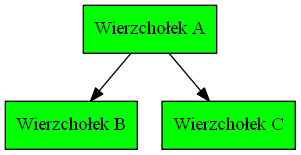
\includegraphics[width=0.3\textwidth]{img/graf.png}
\end{figure}

% SW: Poniższy fragment powinien przenieść Pan od opisu implementacji (nie dotyczy on bezpośrednio Graphviz-a).

%W systemie, którego dotyczy praca magisterska, wykorzystano program dot.exe. Za pomocą funkcji getRuntime klasy Runtime uzyskujemy instancję obiektu klasy Runtime. Na rzecz tego obiektu można następnie wywołać funkcję exec, której argumentem jest tablica łańcuchów znaków zawierająca w pierwszym elemencie ścieżkę do programu (w tym przypadku dot.exe), a w pozostałych elementach argumenty programu. Następnie należy wywołać funkcję waitFor dla obiektu klasy Process, który uzyskujemy w wyniku wywołania funkcji exec.

% SW: Najpierw powinien Pan opisać Graphviz-a (wraz z formatem .dot), a dopiero później bibliotekę służącą do odczytu plików .dot i tworzenia ich reprezentacji obiektowej w Javie.
\section{JPGD - A Java parser for Graphviz documents}

% SW: JPGD jest biblioteką ogólnego przeznaczenia i służy do analizy dowolnych grafów, a nie tylko tych opisujących wytyczne.

% SW: Poniższy opis wydaje się być zbyt szczegółowy, biorąc pod uwagę pomocniczy charakter biblioteki. Poza tym zastosowanie mają wszystkie te uwagi, które sformułowałem w przypadku opisu Choco 3 (dodanie przykładowego kodu źródłowego, zmiana formatowania i zapisu klas/metod).

% SW: Proszę podzielić ten tekst na akaipty -- obecnie mamy jeden wielki akapit obejmujący całą sekcję, a to utrudnia czytanie.

Biblioteka\cite{JPGD} ta służy do konwersji pliku o rozszerzeniu dot na obiekt klasy \texttt{Graph} posiadający listę obiektów klasy \texttt{Node} oraz \texttt{Edge}. Do konwersji wykorzystywany jest obiekt klasy \texttt{Parser}. Klasa \texttt{Parser} posiada funkcję \texttt{parse}, której konstruktor jako parametr przyjmuje obiekt klasy \texttt{FileReader} odwołujący się do określonego pliku o rozszerzeniu dot. W następnym kroku można odczytać obiekt klasy \texttt{Graph} z listy tych obiektów uzyskanej za pomocą funkcji \texttt{getGraphs} (jest to funkcja klasy \texttt{Parser}).

Węzły grafu można odczytać za pomocą funkcji \texttt{getNodes} wywołanej dla obiektu klasy \texttt{Graph}. Krawędzie grafu można natomiast uzyskać za pomocą funkcji \texttt{getEdges}, która również jest funkcją klasy \texttt{Graph}. Węzły oraz krawędzie posiadają atrybuty. Do atrybutów węzłów należy zaliczyć etykietę, kształt, kolor wypełnienia, kolor konturu i grubość linii konturu. Krawędzie posiadają przede wszystkim jeden istotny atrybut – etykietę. Odczytać wartości atrybutów można za pomocą funkcji \texttt{getAttribute}, której argumentem jest nazwa atrybutu. Ustawić wartości atrybutu można natomiast za pomocą metody \texttt{setAttribute}, której pierwszym argumentem jest nazwa atrybutu, a drugim jego wartość. 

Każdy węzeł grafu będącym w formacie dot posiada także swój unikalny identyfikator. Identyfikatory przechowywane są w obiektach klasy Id. Obiekt takiej klasy dla określonego węzła można uzyskać wywołując funkcję \texttt{getId} na rzecz obiektu klasy \texttt{Node}. Ponowne wywołanie funkcji \texttt{getId}, w tym przypadku dla obiektu klasy Id uzyskuje rzeczywisty identyfikator węzła typu \texttt{String}. 

Jeśli chodzi o krawędzie, to posiadają one możliwość odczytania węzła źródłowego oraz docelowego danej krawędzi. Jest to możliwe dzięki wywołaniu funkcji \texttt{getSource} (dla uzyskania węzła źródłowego) oraz \texttt{getTarget} (dla uzyskania węzła docelowego). Dzięki tym funkcjom uzyskujemy obiekt klasy \texttt{PortNode}, z którego następnie możemy uzyskać obiekt klasy \texttt{Node} za pomocą funkcji \texttt{getNode}. Ważną funkcją jest też funkcja \texttt{toString} wywoływana na rzecz obiektu klasy \texttt{Graph}. Pozwala ona na uzyskanie grafu w formacie dot zawierającym zmiany wprowadzone za pomocą metody \texttt{setAttribute} dla obiektów klasy \texttt{Node} lub \texttt{Edge}. 

Poniższy kod źródłowy prezentuje przykładowe wykorzystanie biblioteki JPGD do znalezienia krawędzi wyjściowych węzła n.
\newpage
\begin{verbatim}
public static ArrayList<Edge> getOutEdges(Graph graph, Node n)
{
    ArrayList<Edge> list = new ArrayList<Edge>();
    for(Edge e:graph.getEdges())
    {
       if(e.getSource().getNode()==n)
       {
           list.add(e);
       }
    }
    return list;
}
\end{verbatim}
% SW: Rozumiem, że musiał Pan samodzielnie poprawiać te błędy podczas realizacji pracy. Ten fragment warto przenieśc do podsumowania, gdzie opisuje Pan napotkane problemy.